\chapter{Panoramica del progetto}
\begin{minipage}{12cm}\textit{Nel capitolo verr\`{a} effettuata una breve introduzione ai punti cardine del progetto, verr\`{a} esposto il percorso di progettazione seguito per un suo corretto sviluppo, e illustrato l'utilizzo del software da parte dell'utente.}
\end{minipage}

\vspace*{1cm}
\section{Punti cardine}
In base ai requisiti richiesti, i punti cardine del progetto sono:

\vspace*{0.5cm}
\subsection{HTTP}
\textbf{HTTP}, acronimo di \textit{hypertext transfer protocol}, costituisce il cuore delle azione intraprese dal singolo \textit{bot}.\\
\`E un protocollo a livello applicativo utilizzato per la
trasmissione di informazioni tramite un meccanismo di richiesta/risposta tra \textit{client} e \textit{server}. All'interno del messaggio di richiesta sono definiti diversi campi tra cui, quelli a noi pi\`u tili, il tipo di
richiesta (\textit{GET}, \textit{POST}) e lo \textit{UserAgent}, identificativo del tipo di \textit{client} utilizzato.
Per il nostro scopo, il metodo "\textit{GET}" \`e usato per ottenere il contenuto della risorsa indicata come \textit{URI} (come pu\`o essere il contenuto di una pagina \textit{HTML}). Pu\`o essere:
\begin{itemize}
\item \textbf{assoluto}, ossia quando la risorsa viene richiesta senza altre specificazioni;
\item \textbf{condizionale}, ossia quando la risorsa corrisponde ad un criterio indicato nell'\textit{header};
\item \textbf{parziale}, ossia quando la risorsa richiesta \`e una sottoparte di una risorsa memorizzata.
\end{itemize}
Per quanto riguarda lo \textit{user-agent}, all'interno dell'\textit{header HTTP}, si hanno informazioni riguardanti il tipo di agente utente, cio\`e il tipo di \textit{browser} che sta effettuando la richiesta. Se modificato, permette ad un \textit{hacker} di diventare lo \textit{user-agent} che vuole, potendo cos\`i selezionare i \textit{payload} di software maligni sulla base del tipo di \textit{user-agent}. 
Per il nostro scopo il metodo \textit{GET} \`e stato utilizzato come "assoluto" e si \`e messo a disposizione dell'utente la possibilit\`a di poter modificare lo \textit{user-agent} a proprio piacimento.

\vspace*{0.5cm}
\subsection{Singleton Pattern}
In molte situazioni \`e necessario che venga istanziato un solo esemplare di una data classe. Per esempio: se si ha un riproduttore di file musicali sar\`a bene che esso venga istanziato una sola volta per non ritrovarsi due riproduzioni contemporanee; uno \textit{spooler} di stampa dovrebbe tenere una coda unica anche se ci sono pi\'u
stampanti attive; il manager del file system dovrebbe essere unico, come pure una cache; ecc. Per garantire questa singola istanziazione basta rendere impossible l'uso del costrutto \textit{new} da parte del programma utente e di fornire un metodo indiretto per ottenere una istanza (l'unica) della classe.
A tal fine occorre:
\begin{itemize}
\item dichiarare privato il costruttore, in modo che esso possa essere visto solo dall'interno della classe Singleton e non dal programma utente (ci\`o rende impossibile l'istanziazione di un oggetto dall'esterno della classe Singleton);
\item prevedere il metodo (pubblico) statico e cio\`e di classe, in modo che esso sia comunque visibile. Questo metodo deve istanziare un esemplare se ci\`o non \`e ancora accaduto, oppure restituire l'oggetto gi\'a istanziato in precedenza senza istanziare ulteriori esemplari.
\end{itemize}
Questa seconda scelta \`e quella applicata nel progetto per la creazione e gestione del \textit{logger} e la creazione di uno schedulatore di task.

\vspace*{0.5cm}
\subsection{Schedulatore}
Lo \textit{scheduler} \`e un componente chiave per l'applicazione. \\
Grazie a questo, \`e stato possibile stabilire un ordinamento temporale per l'esecuzione delle azioni del singolo \textit{bot}, cos\`i come specificato dall'utente attraverso i parametri di configurazione. La sua implementazione \`e stata possibile attraverso la creazione di un \textit{executor} a singolo \textit{thread} che schedula comandi da eseguire dopo un certo ritardo o da eseguire periodicamente\footnote{Si noti che se il singolo \textit{thread} termina in maniera anomale durante l'esecuzione, uno nuovo prender\'a il suo posto, se necessario, per eseguire \textit{task} successivi.}. Valori di ritardi pari a 0 o negativi (ma non i periodi) sono trattati come richieste di esecuzione immediata. \\
In sintedi, la schedulazione pu\`o essere cos\`i pensata: il \textit{thread} dello schedulatore assegna i \textit{task} a un \textit{thread} estratto da un \textit{pool}.

\vspace*{0.5cm}
\subsection{ID dei bot e MD5}
I \textit{bot} devono essere univocamente identificabili.\\ 
Questo perch\`e il malintenzionata che vuole effettuare un attacco (per esempio, \textit{DDoS}) deve sapere quanti \textit{bot} ha a disposizione in un certo lasso di tempo. Inoltre, se il malintenzionato decide di affidare un gruppo di \textit{bot} ad un acquirente esterno (per esempio, per condurre una piccola e veloce campagna di \textit{spam}), mantenere un conteggio della potenza di attacco che possono essere offerti \`e necessario per accordarsi sul prezzo. Per garantire l'unicit\'a dell'identificativo di ciascuno, si \`e deciso di legare l'hardware della macchina al suo sistema operativo tramite\textit{checksum MD5} per ottenere una stringa a 32 caratteri che \`e utilizzata come identificativo.\\
Si noti come questo \`e stato fatto per una integrazione con un futuro sviluppo del progetto.

\vspace*{0.5cm}
\subsection{Parsing}
Per \textit{parsing} di una stringa di caratteri si intende l'analisi della stessa per trovare \textit{token}, oggetti o \textit{pattern} per crearne una struttura.\\
Nel progetto era importante definire un \textit{pattern} per i parametri di configurazione, per rivelare la loro correttezza e capire se si trattasse di un campo facoltativo o meno, per poter cos\`i capire se la computazione dovesse fermarsi l\`i. Quanto detto \`e stato applicato sia in lettura, sia in scrittura: questo perch\`e i parametri di configurazione possono essere anche salvati su un file di testo.

%\vspace*{0.5cm}
%\subsection{Multithreading}
%Al fine di garantire la concorrenzialit\'a, vi \`e la necessit\'a di servire separatamente ogni \textit{GET}, scelta \`e stata dettata dall'importanza di ridurre il carico della piattaforma. D'altro canto, il %\textit{multithreading} presenta il problema degli accessi simultanei a variabili e segmenti di codice condivisi dai vari thread (zone critiche). In sporadici casi, questo ha causato dei problemi di corruzione della memoria di cui non \`e stato possibile risalire all'origine.
%Il multithreading \`e stato utilizzato in questo modo: una volta presentata la richiesta, viene creato un nuovo thread, responsabile della richiesta, permettendo cos\`i al flusso principale di effettuarne altre. I thread sono creati tramite l'invocazione della funzione TODOTODOTODO.\\

\vspace*{0.5cm}
\subsection{Multi-piattaforma}
Quando si parla di un programma multi-piattaforma si intende un programma che sia in grado di funzionare correttamente su diversi sistemi operativi.\\
A tale fine, l'esecuzione di istruzioni "macchina-dipendenti" (come, per esempio, la generazione dell' ID del bot che dipende sia dall'hardware che dal sistema operativo) appariranno all'utente in maniera totalmente trasparente per sistemi operativi come OSX, Windows o Linux. 

\vspace*{0.5cm}
\section{Piattaforma di sviluppo, Swing, Awt}
NetBeans \`e un ambiente di sviluppo integrato (\textit{IDE} -  \textit{Integrated Development Environment}) multi-linguaggio, scelto dalla Oracle Corporation come \textit{IDE} ufficiale da contrapporre al pi\'u diffuso Eclipse.\\
NetBeans utilizza due componenti principali: la piattaforma, che comprende una serie di librerie per fornire gli elementi base dell'\textit{IDE} come presentazione dei dati e interfaccia utente, e l'\textit{IDE} vero e proprio, che permette di gestire il controllo e le funzionalit\'a offerte dalla piattaforma. NetBeans utilizza \textit{Abstract Window Toolkit} (\textit{AWT}), un insieme di API realizzate da Sun che permettono agli sviluppatori di modellare le interfacce grafiche delle finestre, pulsanti e altri elementi visuali. \textit{AWT} fornisce gli elementi grafici base che dipendono dalla piattaforma utilizzata, mentre per gli aspetti di alto livello come gestione di colori e interazione con l'utente \`e usata la libreria Swing.

\vspace*{1cm}
\section{Build your own botnet}
Questa sezione tratta del programma e della sua architettura, nonch\`e delle scelte implementative rilevanti e dei casi d'uso principali.

\vspace*{0.5cm}
\subsection{Struttura del progetto}
Il progetto \`e composto da diverse classi:
\begin{itemize}
\item \textbf{ByobComm}, responsabile del metodo GET del protocollo HTTP;
\item \textbf{ByobSingleton}, responsabile del \textit{log} delle azioni intraprese, delle informazioni della macchina dell'utente e dello \textit{scheduling} dei \textit{task} da effettuare;
\item \textbf{ByobTask}, implementa l'interfaccia \textit{Runnable} per il \textit{multithreading};
\item \textbf{Byob\_v1}, avvia il programma e l'interfaccia grafica;
\item \textbf{GUI}, responsabile di tutto quello che riguarda la creazione e gestione della \textit{Graphic User Interface} (quindi, componenti, loro visibilit\'a, loro aspetto e la loro abilitazione per l'uso);
\item \textbf{Parser}, responsabile per la creazione di file, lettura e scrittura dei parametri di configurazione inseriti dall'utente, nonch\`e del loro \textit{splitting} e della loro conversione nel giusto tipo di dato;
\item \textbf{Tools}, contenente varie funzioni e vari metodi che non appartenevano a nessun'altra classe;
\item \textbf{URLDetails}, contenente i dati (parametri di configurazione) del singolo \textit{task} da effettuare.
\end{itemize} 

\vspace*{0.5cm}
\subsection{ByobComm}
La classe \textit{ByobComm} gestisce tutto quello che riguarda il protocollo HTTP.\\
Prima di creare una connessione si controlla che tipo di parametri di configurazione ha inserito l'utente e se impattano sull'apertura della connessione. Uan volta istanziato l'oggetto (con o senza \textit{proxy}, in base all'input dell'utente), la connessione \`e aperta, si setta il metodo di tipo \textit{GET}, la codifica dell'\textit{header} e lo \textit{user-agent} (se \`e stato fornito). A questo punto si estrae il codice di risposta, prima di chiudere la connessione, che viene analizzato all'interno del programma per i fini progettuali. \\
Con lo stesso approccio, si era originariamente pensato di creare una funzione booleana per il controllo dell'\textit{URL} inserito dall'utente subito dopo aver premuto il pulsante "\textit{Push}": purtroppo impattava sulle prestazioni dell'interfaccia grafica (il pulsante rimaneva cliccato finch\`e non era chiusa la connessione).

\vspace*{0.5cm}
\subsection{ByobSingleton}
Come suggerisce il nome, la classe \textit{ByobSingleton} \`e la responsabile per il \textit{singleton} che si occupa di creare il \textit{log} per la trascrizione di:
\begin{itemize}
\item contatti e parametri di configurazione;
\item \textit{timestamp} di contatto delle URL ed dettaglio delle URL contattate;
\item informazioni relative al Sistema Operativo e al/i browser presenti sulla postazione su cui il software \`e installato.
\end{itemize}
oltre il \textit{log}, la classe gestisce lo schedulatore dei \textit{task}, di cui si \`e parlato precedentemente.

\vspace*{0.5cm}
\subsection{ByobTask}
La classe \textit{ByobTask} si occupa della definizione del singolo \textit{thread} (o \textit{task}).\\
\`E stata focalizzata l'attenzione sul \textit{polling} con intervallo esteso e casuale per verificare se non sono pi\'u rispettate le \textit{sleep condition}: la casualit\'a \`e stata dettata dal fatto che se il contatto avveniva sempre alla stessa ora in cui veniva schedulato poteva destare sospetti e, grazie alla sua semplicit\'a, permette di evitare di dover ogni volta controllare quale/i \`e/sono la/le \textit{sleep condition}.

\vspace*{0.5cm}
\subsection{Byob\_v1}
La classe in esame non \`e nient'altro che la responsabile dell'invocazione della \textit{GUI} (e del settaggio del titolo, assieme alla sua posizione per far in modo che appaia al centro dello schermo, indipendentemente dalla sua grandezza) ed \`e stata utilizzata a scopo di testing per trovare i giusti comandi da terminale per l'individuazione dei browser, cos\`i come richiesti nell'estensione del documento di progetto.

\vspace*{0.5cm}
\subsection{GUI}
\begin{figure}[!htb]
        \centering
		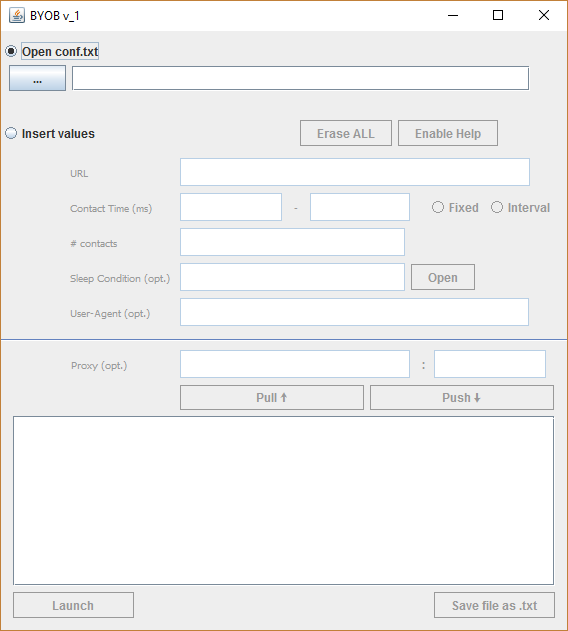
\includegraphics[width=0.7\linewidth]{./imgs/gui}
        \caption{Apertura di un file di configurazione}
        \label{apertura}
        \vspace*{0.5cm}
\end{figure}

La classe \textit{GUI} \`e il cuore dell'applicazione e rappresenta l'interfaccia grafica con cui l'utente fornisce i parametri di configurazione.\\
A prima vista, l'interfaccia pu\`o risultare complicata, ma si \`e cercato di rendere la modalit\'a di fruizione pi\`u intuitiva possibile, attraverso piccole azioni per il suo utilizzo e con una grafica molto semplice, dato che ci si \`e soffermati pi\'u sulla sua logica di funzionamento.
Le azioni iniziali che l'utente pu\`o intraprendere, tramite le \textit{checkbox}, sono due:
\begin{enumerate}
\item Aprire un file di configurazione gi\'a in possesso dell'utente;
\item Inserire manualmente i parametri di configurazione.
\end{enumerate}

\begin{figure}[!htb]
        \centering
		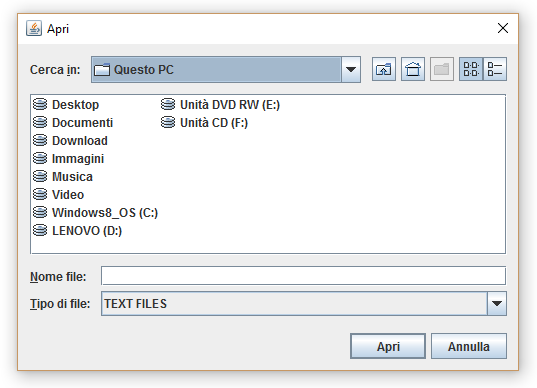
\includegraphics[width=0.6\linewidth]{./imgs/scelta1}
        \caption{Apertura di un file di configurazione}
        \label{apertura}
\end{figure}
L'apertura di un file di configurazione \`e riconducibile all'apertura di un qualsiasi file, gesto oramai assimilato nella vita di tutti i giorni. Cliccando sull'apposito pulsante "...", viene aperto il textit{JFileChooser}, un semplice meccanismo di scelta a disposizione dell'utente (una sorta di \textit{file explorer} per muoversi tra file e cartelle del \textit{file system}). Ad esso \`e stato applicato un filtro con cui sono visibili solo cartelle e file di testo: questo perch\`e i parametri di configurazione vengono letti esclusivamente da file con estensione ".txt".\\

\begin{figure}[!htb]
        \centering
		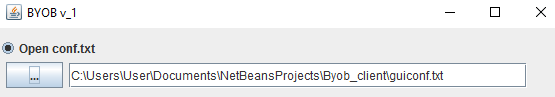
\includegraphics[width=0.7\linewidth]{./imgs/scelta11}
        \caption{Scelta del file di configurazione}
        \label{scelta}
\end{figure}
Una volta selezionato, il path del file scelto apparir\'a nella casella di testo relativa, sbloccando il pulsante "Launch" per il \textit{run} dell'applicazione.

\begin{figure}[!htb]
        \centering        
        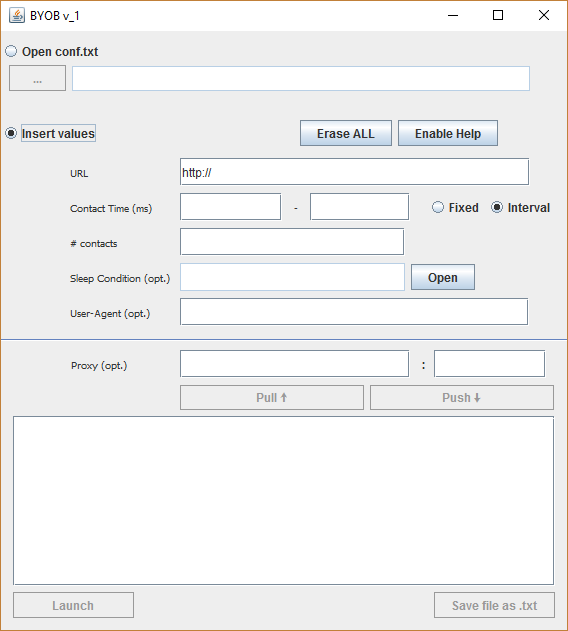
\includegraphics[width=0.7\linewidth]{./imgs/gui2}
        \caption{Inserimento manuale parametri di configurazione}
        \label{inserimento}
\end{figure}

\newpage
L'altra opzione \`e quella dell'inserimento manuale dei parametri di configurazione.\\
Tali parametri sono:
\begin{itemize} 
\item \textbf{URL} da contattare;
\item \textbf{Contact time}, ossia la periodicit\'a di contatto che pu\'o essere:
\begin{itemize}
\item [-] Fissa ("\textit{Fixed}");
\item [-] Invervallo ("\textit{Interval}"), cio\`e all'interno di un intervallo temporale;
\end{itemize} 
\item \textbf{\# contacts}, ossia il numero massimo di contatti per ciascuna URL;
\item \textbf{Sleep conditions} (opzionale), ossia l'insieme di condizioni temporali in cui non viene svolta alcuna azione; sono state divise in condizioni sui giorni e condizioni sulle ore della singola giornata, ognuna caratterizzata da una lettera dell'alfabeto o ad una stringa vuota nel caso di nessuna restrizione:
\begin{figure}[!htb]
        \centering
		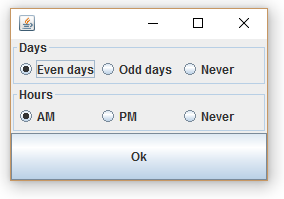
\includegraphics[width=0.4\linewidth]{./imgs/sleep}
        \caption{Sleep conditions}
\end{figure}
\begin{itemize}
\item [-] Condizione sui giorni pari (E), sui giorni dispari (O), nessuna restrizione;
\item [-] Condizione sulle prime dodici ore (A), condizione sulle ultime 12 ore (P), nessuna restrizione;
\end{itemize}
\item \textbf{User-Agent} (opzionale), ossia la modifica da apportare allo User-Agent del protocollo HTTP;
\item \textbf{Proxy} (opzionale), ossia l'indirizzo e porta di un proxy pubblico da utilizzare.
\end{itemize} 

Una volta inseriti nelle relative caselle di testo, il pulsante "\textit{Push}" permette di visualizzare tali parametri (come apparirebbero se fossero stati scritti sul file di configurazione) nell' area di testo sottostante: si noti come, inserendo altri parametri, essi vengano appesi a quelli gi\'a presenti. Il pulsante "\textit{Pull}" permette di estrarre dall'area di testo l'ultimo inserimento effettuato per una eventuale modifica dei parametri non correttamente inseriti.
\begin{figure}[!htb]
        \centering
		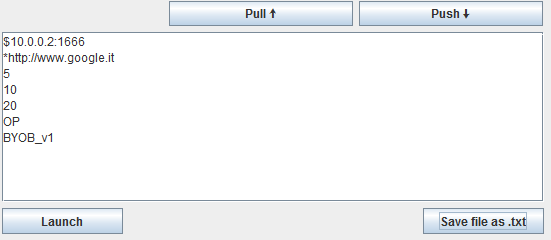
\includegraphics[width=0.6\linewidth]{./imgs/textarea}
        \caption{Push - Inserimento dell'input nell'area di testo}
        \vspace*{0.5cm}
\end{figure}

L'inserimento manuale ha il fine di salvare tutti i parametri di configurazione all'interno di un file di testo (azione svolta dal pulsante "Save file as .txt"), con un approccio simile a quello utilizzato per l'apertura del file di configurazione, cio\`e attraverso il textit{JFileChooser}.

\paragraph{GUI user-friendly}
Per rendere il tutto semplice e a portata di qualsiasi utente, il \textit{toogle} "\textit{Enable Help}" permette di invocare dei \textit{tooltips} sulle caselle di testo per meglio capire che dato inserire e in che formato. Nell'esempio fornito, per sapere come correttamente inserire il parametro \textit{URL}, basta posizionarsi col mouse sulla casella di testo corrispondente e attendere qualche secondo.
\begin{figure}[!htb]
        \centering        
        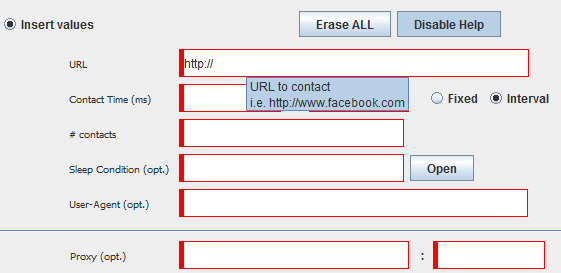
\includegraphics[width=0.7\linewidth]{./imgs/help}
        \caption{Utilizzo dell'help}
        \label{help}
\end{figure}
\\Per quanto riguarda il pulsante "\textit{Erase ALL}", la sua implementazione \`e nata dalla volont\'a di fornire all'utente un metodo veloce per cancellare ogni inserimento nelle caselle di testo nel caso di molteplici errori.\\
Infine si \`e scelto di fornire un \textit{warning message}, con l'approccio di un \textit{pop-up}, in caso di errato e/o mancato inserimento di uno o pi\'u parametri tramite il pulsante "\textit{Push}": l'utente, a questo punto, pu\'o decidere se tornare indietro e correggere da solo l'errore oppure utilizzare dei valori di \textit{default} per i parametri di configurazione.
\begin{figure}[!htb]
        \centering        
        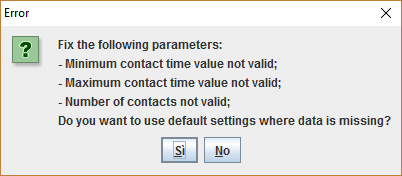
\includegraphics[width=0.6\linewidth]{./imgs/warning}
        \caption{Esempio di messaggio d'errore per dati mancanti e/o errati}
        \label{warningMessage}
\end{figure}

\vspace*{0.5cm}
\subsection{Parser}
La classe \textit{Parser} si occupa di tutti gli aspetti legati al controllo dell'\textit{input}, sia dal punto di vista sintattico che dal punto di vista alfanumerico, ma anche la correttezza di \textit{pattern}, come nel caso venga inserito un indirizzo IP per il \textit{proxy}. Altre responsabilit\'a della classe sono:
\begin{itemize}
\item lettura e scrittura del file contenente i parametri di configurazione;
\item creazione di una lista di istanze della classe \textit{URLDetails}, una per ciascun contatto da effettuare;
\item conversione dei parametri di configurazione nel tipo corretto (per fornire un esempio, il numero di contatti da stringa a intero);
\item controllo della validit\'a di ciascun parametro di configurazione (se il parametro \`e un numero, se gli estremi degli intervalli sono uno maggiore dell'altro, \dots ).
\end{itemize}

\vspace*{0.5cm}
\subsection{Tools}
La classe \textit{Tools} contiene al suo interno, tra varie funzioni e vari metodi, la generazione dell' identificativo del \textit{bot}.\\
Tale generazione \`e effettuata tramite la ricerca del sistema operativo della macchina ospitante per poi lanciare, tramite riga di comando, delle istruzioni con cui ottenere dati riguardanti l'\textit{hardware} della stessa. Queste informazioni  sono poi "date in pasto" ad un funzione \textit{hash} con cui \`e generato l'ID. La decisione di utilizzare entrambe le informazioni, sia \textit{hardware} che \textit{software} \`e stata dettata dalla volont\'a di ridurre le possibilit\'a di ID uguali, grazie all' indirizzo \textit{MAC} univoco della macchina e al sistema operativo che pu\`o trovarsi su pi\'u macchine differenti.
La funzione \textit{hash} usata \`e MD5, fornita dalla classe \textit{MessageDigest}, perch\`e \`e veloce da generare e non si avevano grosse pretese di sicurezza (non si tratta di una password ma bens\`i di un identificativo che servir\'a al \textit{botmaster} per capire quante unit\'a ha a disposizione per un eventuale attacco).\\
Questa classe si occupa anche della schedulazione dei \textit{task}, tramite l'unica istanza della classe \textit{ByobSingleton}.
Altri metodi e funzioni della classe hanno lo scopo trovare informazioni sulla macchina ospitante (sistema operativo, architettura, browser installati, lanciare istruzioni da riga di comando) ed effettuare i controlli per la generazione del \textit{warning message} della classe GUI.

\vspace*{0.5cm}
\subsection{URLDetails}
\textit{URLDetails} \`e la classe che contiene tutte le informazioni inserite dall'utente per ciascun contatto che il \textit{bot} deve effettuare. Oltre agli attributi, che coincidono con i parametri di configurazione forniti dall'utente, mette a disposizione i metodi getXX e setXX (dove XX \`e il parametro di configurazione) per recuperare e settare il loro valore.